Currently Kubernetes implemenents horizontal pod auto-scaling.
As this title suggests, auto-scaling in
Kubernetes invovles creating an autoscaler for a specific replication
controller such that the replica pods handling the requests load-balanced by the service
operate within a specified resource range. Kubernetes
implementation of auto-scaling is referred to as horizontal because
auto-scaling occurs by creating replicas of each pod and then dividing the work
among these replicas, as opposed to expanding the resources of any single pod.
While not yet implemented, Kubernetes reliance upon containers means vertical
auto-scaling is a possibility in the near future, as there are a variety of
methods for increasing the resources available to a container without stopping
execution \cite{docker-up-and-running}.

As was distinguished in the background section, Kubernetes currently implements reactive
feedback control auto-scaling, which is defined as when auto-scaling occurs to
ensure the preservation of a certain state. Reactive auto-scaling can be
visualized through Figure \ref{fig:reactive-autoscale}.
This operation becomes clear when examining
the execution of the horizontal pod autoscaler. To begin, the autoscaler
operates as a control loop, as it queries pods at a set interval to determine
their current resource utilization, and performs auto-scaling actions depending on the
resulting utilization. At the start of this thesis, the only resource on which it is possible to
determine auto-scaling behavior is CPU utilization percentage, but possible
resources could conceivably expand to include percent memory utilized, percent
network bandwidth used, etc. Based on the average CPU utilization percentage, the
auto-scaler will create or delete replica pods to ensure average CPU utilization
percentage is within the target range the user specificed when creating the
autoscaler. The algorithm for determining the correct number of replica pods
will be discussed in detail in the next section. The final implementation detail
is that, in order to ensure auto-scaling is not attempted to frequently, once a
scale up or scale down happens, no more auto-scaling will occur for a constant
interval.\footnote{This interval is currently five minutes from the most recent
rescaling for scale-down and three minutes from the most recent rescale for
scale-up.} This waiting time ensures auto-scaling can actually take effect
before it is potentially attempted again \cite{k8s-horizontal-pod-autoscaler-user-guide}.

\begin{figure}[!h]
  \centerline{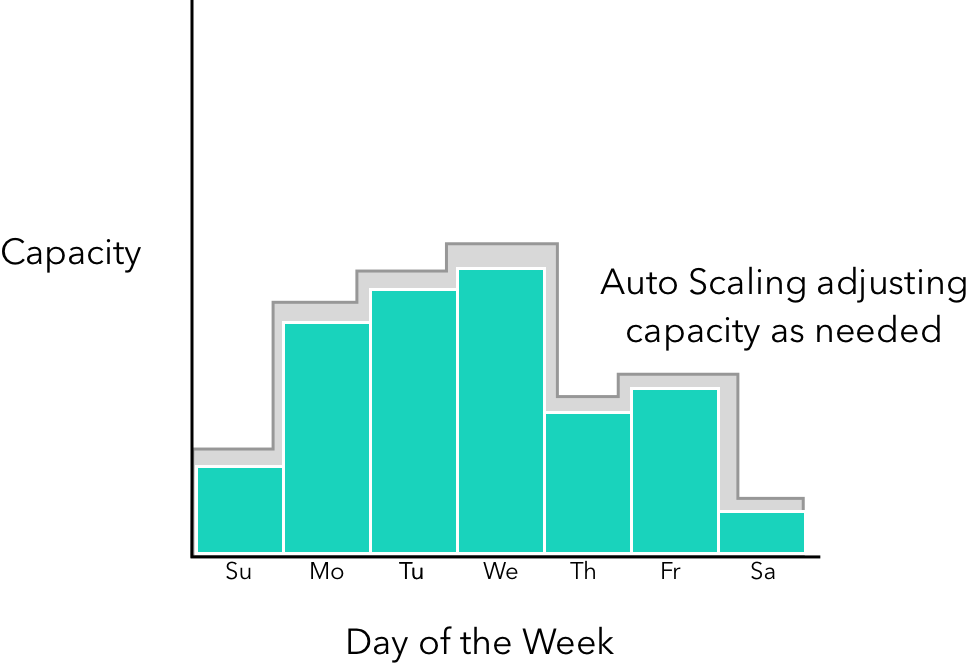
\includegraphics[scale=.25]{reactive-autoscale}}
  \caption{A Reactive Auto-scaled Application}
  \label{fig:reactive-autoscale}
\end{figure}
